\documentclass[tikz,border=1pt]{standalone}
\input{figpreamble}
\begin{document}
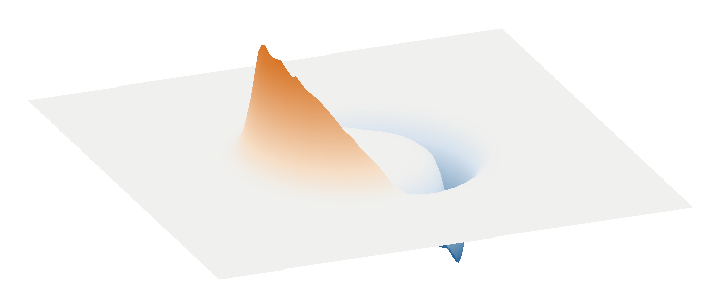
\begin{tikzpicture}[declare function={rr(\x,\y)=sqrt(\x*\x+\y*\y)+1e-9; sechsq(\a)=1/(cosh(\a)^2); fp(\r)=8*(sechsq(8*(\r+1)) - sechsq(8*(\r-1)))/(2*tanh(8));}]
\begin{axis}[hide axis, view={-22}{38}, xmin=-2.6, xmax=2.6, ymin=-2.6, ymax=2.6, zmin=-4.2, zmax=4.2, clip=false, width=285pt, height=225pt, colormap={diverge}{rgb255(0cm)=(29,91,143) rgb255(4cm)=(214,226,238) rgb255(5cm)=(240,240,238) rgb255(6cm)=(246,221,196) rgb255(10cm)=(214,112,32)}, point meta min=-4, point meta max=4]
\addplot3[surf, shader=interp,  samples=71, samples y=71, domain=-2.6:2.6, y domain=-2.6:2.6] {x/rr(x,y)*fp(rr(x,y))};
\end{axis}
\end{tikzpicture}
\end{document}
